\chapter{Convex Conjugates}
\label{chap:convex_conjugates}

\section{Definition and properties}

This chapter introduces a concept that is deeply connected to subgradients and
proximal mappings (as covered in the last two chapters), and to duality theory
(as will be covered next). In fact, just as with subgradients, proximal
mappings, and duality, the topic of the current chapter is simultaneously simple
and elementary, as well as highly nontrivial and powerful.    

Given a function $f : \R^d \to [-\infty, \infty]$, its \emph{convex conjugate}
$f^*$ (also simply called its conjugate) is another function on $\R^d$ defined
as        
\index{convex conjugate}
\index{Legendre-Fenchel transform}
\begin{equation}
\label{eq:conjugate}
f^*(u) = \sup_x \, \Big\{ u^\T x - f(x) \Big\}.
\end{equation}
The mapping from $f \mapsto f^*$ is also called the \emph{Legendre-Fenchel
  transform}. At the outset, we remark that $f^*$ is always convex, by the
partial supremum rule in Property \parref{par:function_supremum} (the map
$u \mapsto u^\T x - f(x)$ is convex, indeed, it is affine, for each $x$). To 
be clear, this is true regardless of the convexity of $f$, which is why $f^*$ is 
called its convex conjugate.  

A useful interpretation of $f^*$ is as follows: at each point $u$, the value
$f^*(u)$ is the maximum gap between a linear function with ``slope'' $u$ and
$f$. Figure \ref{fig:conjugate} gives an illustration. This interpretation
suggests that there may be some interesting geometry at play that underlies the
convex conjugate, which we revisit shortly when we discuss double conjugation.      

\begin{figure}[tb]
\centering
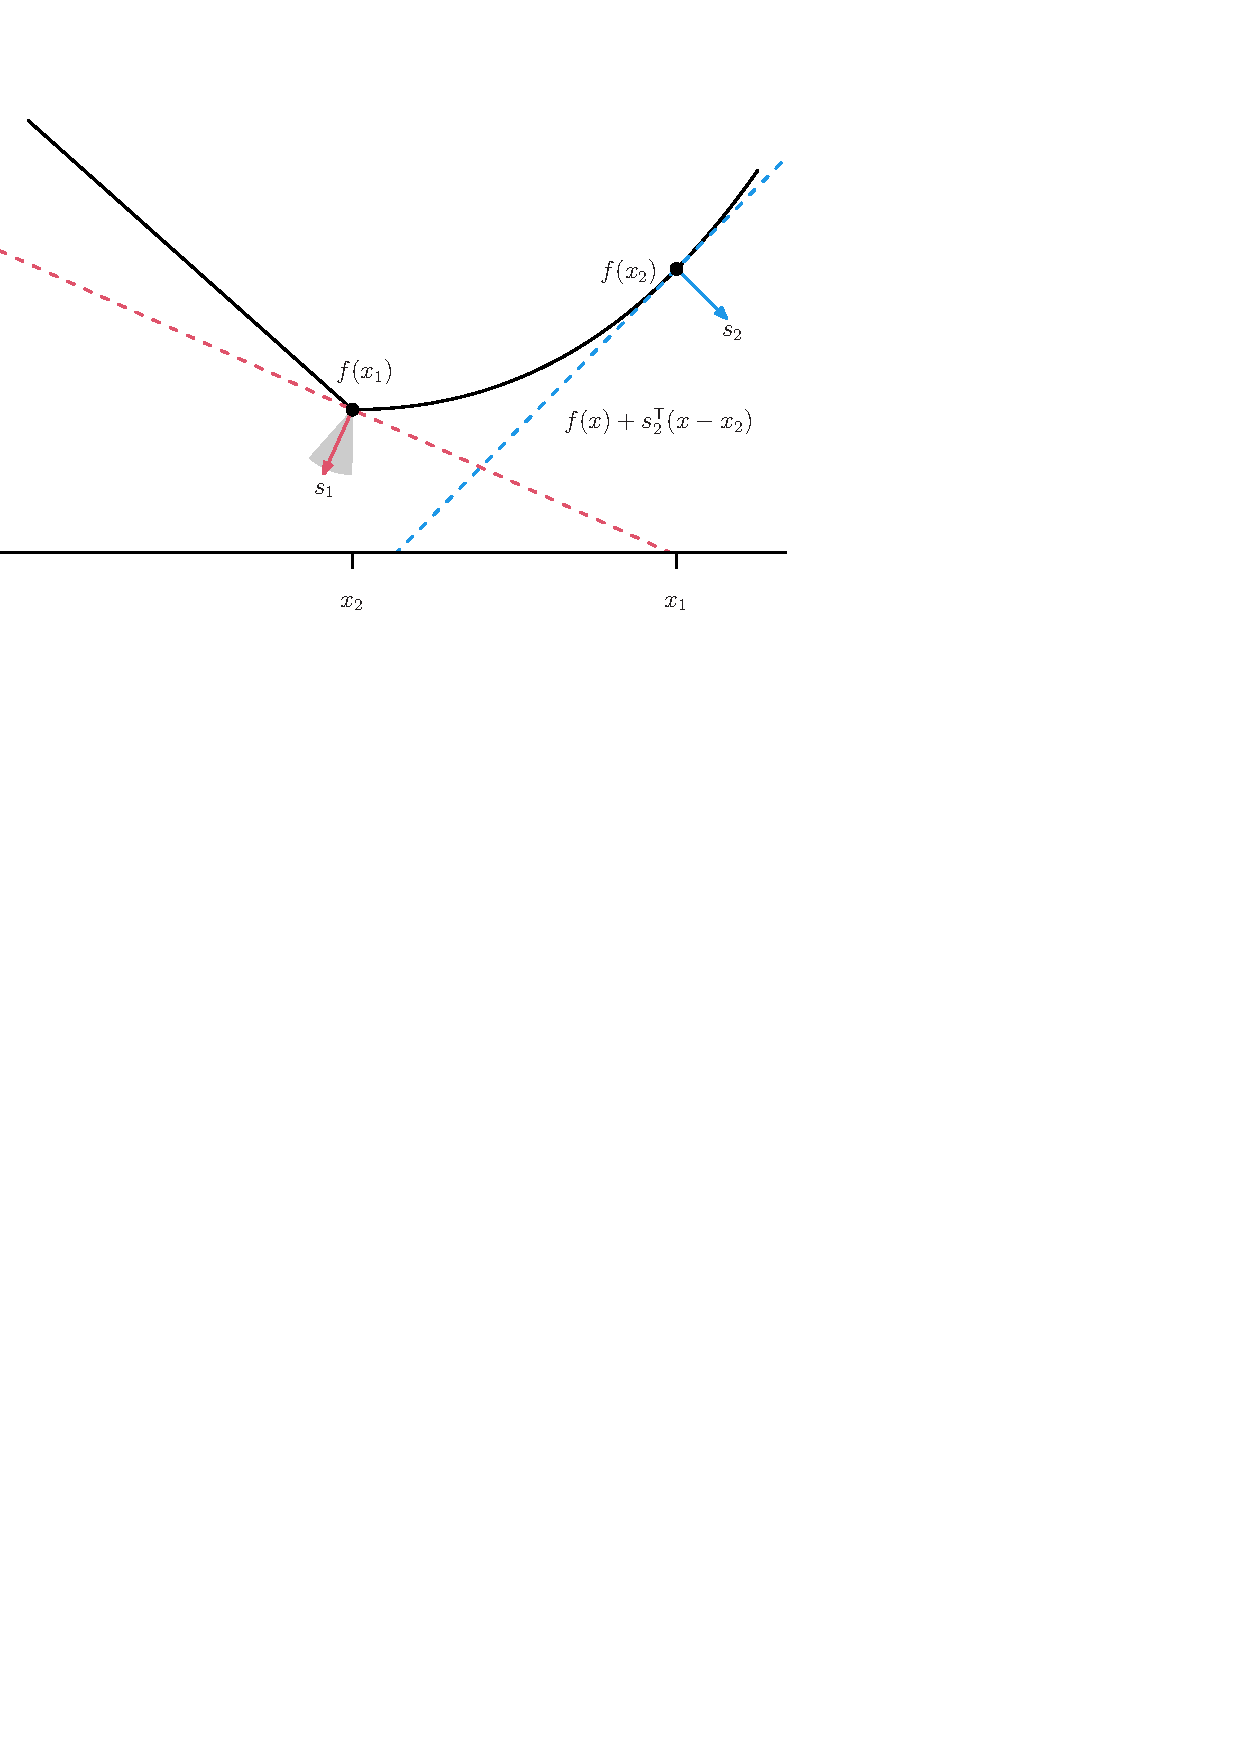
\includegraphics[width=0.7\textwidth]{fig/subgradient.pdf}
\caption{The conjugate $f^*$ at $u$ is the maximum gap between a linear function
  with slope $u$ and $f(x)$, which is illustrated by the dotted line. The double
  conjugate $f^{**}$ is the pointwise supremum of all affine minorants to $f$,
  that is, the greatest closed convex minorant to $f$, which is illustrated by
  the dashed line.}
\label{fig:conjugate}
\end{figure}

Next we describe important properties of convex conjugates. Henceforth we
generally assume that $f \not= \infty$ ($\dom(f) \not= \emptyset$) to avoid
trivialities when studying convex conjugates.      

\paragraph{Fenchel's inequality.}

For any $u$, observe that by the definition of the convex conjugate
\eqref{eq:conjugate} it holds that $f^*(u) \geq u^\T x - f(x)$, for any
$x$. Rearranging yields what is called \emph{Fenchel's inequality}, 
\index{Fenchel's inequality}
\begin{equation}
\label{eq:fenchel_inequality}
f(x) + f^*(u) \geq x^\T u, \quad \text{for all $x,u$}.
\end{equation}
Equality holds in \eqref{eq:fenchel_inequality} if and only if $x$ achieves the
supremum in \eqref{eq:conjugate}. As we show next, this can be further
characterized using subgradients of $f$.   

\paragraph{Subgradient equivalences.}

The supremum in \eqref{eq:conjugate} is attained at $x$ if and only if $x$
solves  
\[
\minimize_x \quad f(x) - u^\T x,
\]
which for convex $f$ is equivalent to $0 \in \partial f(x) - u$, that is, $u \in 
\partial f(x)$, using subgradient optimality. (Note that we use convexity 
of $f$ to split the subdifferential of a sum into a sum of subdifferentials, by 
Property \parref{par:subgradient_sum}.)  Meanwhile, by the rule for subgradients
of a partial supremum (Property \parref{par:subgradient_supremum}) we know that
$\partial f^*(u)$ contains all points of the form 
\[
\nabla_u \big( u^\T x - f(x) \big) = x,
\]
such that $x$ that achieves the supremum in \eqref{eq:conjugate}. In fact, if
$f$ is \emph{closed} and convex, then using the fact that $f^{**} = f$, to be 
established below, we can conclude that this describes \emph{all} of the
elements of $\partial f^*(u)$ (Exercise \ref{ex:conjugate_subgradients}). The 
next result records these equivalences. 

\index{convex conjugate!subgradients}
\begin{Theorem}
For closed and convex $f$ with nonempty domain, the following statements are all 
equivalent:
\begin{enumerate}[label=(\roman*)]
\item $x$ achieves the supremum in \eqref{eq:conjugate};
\item $f(x) + f^*(u) = x^\T u$;
\item $u \in \partial f(x)$;
\item $x \in \partial f^*(x)$.
\end{enumerate}
\end{Theorem}
\vspace{-3pt}

\paragraph{Double conjugation.}

The conjugate of $f^*$ is known as the \emph{double conjugate} of $f$ and
denoted $f^{**}$. Simply applying the definition \eqref{eq:conjugate} with $f^*$
in place of $f$, we get 
\index{convex conjugate!double}
\begin{equation}
\label{eq:double_conjugate}
f^{**}(x) = \sup_u \, \Big\{ x^\T u - f^*(u) \Big\},
\end{equation}
and by the same rationale given previously, we note that $f^{**}$ is always
convex. Applying Fenchel's inequality \eqref{eq:fenchel_inequality}, that is,
$f^*(u) \geq x^\T u - f(x)$, to the term inside the supremum gives    
\[
f^{**} \leq f,
\]
or in other words, the double conjugate $f^{**}$ minorizes the original function
$f$. In fact, the double conjugate function $f^{**}$ is not just any (convex)
minorant of $f$, it is the pointwise supremum of all affine minorants of $f$
(Exercise \ref{ex:double_conjugate_affine_minorant}):       
\begin{equation}
\label{eq:double_conjugate_affine_minorant} 
f^{**}(x) = \sup \{ g(x) : \text{$g$ is affine, and $g \leq f$} \}, \quad
\text{for all $x \in \dom(f)$}. 
\end{equation}
See Figure \ref{fig:conjugate} again for an illustration. Lastly, an important
special reduction occurs for closed and convex $f$: in this case, we get   
\begin{equation}
\label{eq:double_conjugate_reduction}
f^{**} = f.
\end{equation}
Exercises
\ref{ex:affine_minorant_revisited}--\ref{ex:double_conjugate_reduction} walk
through the proof of this and related facts.

\medskip

\begin{Example}
Below are examples of convex conjugates for a few well-known functions of
interest. The calculations for most are straightforward, and for others we defer
the details to exercises. 

\begin{enumerate}[label=\alph*., ref=\alph*]
\item For $f(x) = \frac{1}{2} x^\T Q x$, where $Q \succ 0$, its conjugate is
  $f^*(u) = \frac{1}{2} u^\T Q^{-1} u$.

\item For $f(x) = \sum_{i=1}^d x_i \log(x_i)$, its conjugate is $f^*(u) =
  \sum_{i=1}^d \exp(u_i - 1)$. 

\item \parlab{xa:characteristic_function_conjugate}   
  For $f = I_C$, the characteristic function of an arbitrary set $C$, its
  conjugate is \vphantom{$\sum_{i=1}^d$} 
  \index{characteristic function!conjugate}
  \[
  f^* = h_C,
  \]
  where recall \smash{$h_C(u) = \sup_{x \in C} \, u^\T x$} denotes the support
  function corresponding to $C$.  

\item \parlab{xa:support_function_conjugate} 
  For $f = h_C$, the support function corresponding to a closed, convex, and
  nonempty set $C$, its conjugate is (Exercise
  \ref{ex:support_function_conjugate}):    
  \index{support function!conjugate} 
  \[
  f^* = I_C,
  \]
  the characteristic function of $C$. 

\item \parlab{xa:norm_conjugate}  
  For $f(x) = \|x\|$, where $\|\cdot\|$ is an arbitrary norm, its conjugate is
  (Exercise \ref{ex:norm_conjugate}):  
  \index{norm!conjugate}
  \[
  f^* = I_{\{u \,:\, \|u\|_* \leq 1\}},
  \]
  the characteristic function of the unit ball in the dual norm
  $\|\cdot\|_*$. (Chapter \ref{sec:dual_norms} will develop the connection
  between $\|\cdot\|$ and $\|\cdot\|_*$ in more detail.)  
\end{enumerate}
\end{Example}

\section{Conjugate calculus}

should check rockafellar and bertsekas

\section{Conjugates and smoothness*}
\label{sec:conjugates_smoothness}

discuss relationships between smoothness of f, f* 

define Legendre function (essential smoothness, essential strict convexity).
gradient map is a homeomorphism (with inverse being graident of conjugate) 

\section{Proximal connections*}

\subsection{Moreau decomposition}
\label{sec:moreau_decomposition}

\subsection{Moreau envelope, revisited}

Chapters 11 and 12 or Rockafellar masterful geometric treatment of
conjugacy. Exercise \ref{ex:affine_minorant_revisited} gives a glimpse of what
the geometric view can provide

The connection between the moreau envelope and regularization is due to Hedy
Attouch in 1977  

infimal convolution and conjugates and addition

relationship between conjugates and moreau envelopes, which shows it as a form
of smoothing 

\begin{xcb}{Exercises}
\begin{enumerate}[label=\thechapter.\arabic*]
\settowidth{\leftmargini}{0.00.\hskip\labelsep}
\index{convex conjugate!subgradients}
\item \label{ex:conjugate_subgradients}
  In this exercise, we examine subgradients of the conjugate function
  \eqref{eq:conjugate}.  

\begin{enumerate}[label=\alph*.]
\item Show that $x \in \partial f^*(u)$ for any $x$ that achieves the supremum
  in \eqref{eq:conjugate}. Hint: recall the rule in Property
  \parref{par:subgradient_supremum}. 

\item When $f$ is closed and convex, show further that $x \in \partial f^*(u)$
  if and only if $x$ achieves the supremum in \eqref{eq:conjugate}. Hint: first
  show $x \in \partial f^*(u)$ if and only if $u$ achieves the supremum in
  \eqref{eq:double_conjugate}, by subgradient optimality. Then use the fact that
  $u$ achieves the supremum in \eqref{eq:double_conjugate} if and only if
  $f^{**}(x) + f^*(u) = x^\T u$. Lastly, reinterpret the last condition using
  the fact that $f^{**} = f$ for closed convex $f$. 
\end{enumerate}

\item \label{ex:double_conjugate_affine_minorant}
  In this exercise, we establish the fact in
  \eqref{eq:double_conjugate_affine_minorant}, for $x \in \dom(f)$, by proving
  separately that the left-hand side is at most and at least the right-hand
  side.    

\begin{enumerate}[label=\alph*.]
\item Prove that $f^{**}(x) \geq \sup \{ g(x) : \text{$g$ is affine, and $g \leq
    f$} \}$. Hint: if $g(x) = u^\T x + b$ satisfies $g \leq f$, then show that
  $f^*(u) \leq -b$, and thus $f^{**}(x) \geq u^\T x + b = g(x)$. 
  
\item Prove that $f^{**}(x) \leq \sup \{ g(x) : \text{$g$ is affine, and $g \leq
    f$} \}$. Hint: observe that $f^{**}(x)$ is the supremum of $g(x)$ over all
  affine minorants $g$ that take the form $g(y) = u^\T y - f^*(u)$.  
\end{enumerate}

\item \label{ex:affine_minorant_revisited}
  This exercise proves a refined version of the fact from Exercise
  \ref{ex:affine_minorant}: for closed and convex $f$,  
  \begin{equation}
  \label{eq:affine_minorant_revisited}
  f(x) = \sup \{ g(x) : \text{$g$ is affine, and $g \leq f$} \}, \quad \text{for
    all $x \in \dom(f)$}.
  \end{equation}
 % Theorem 12.1 in Rockafellar (1970)
  Note that we really only need to prove that the equality holds for $x \in
  \dom(f) \setminus \relint(\dom(f))$, as the result was already established on
  $\relint(\dom(f))$ (using the existence of subgradients) in Exercise  
  \ref{ex:affine_minorant}. Nonetheless, in this exercise we will adopt a
  different, geometric approach to establishing
  \eqref{eq:affine_minorant_revisited} that seamlessly applies to all $x \in
  \dom(f)$.    

\begin{enumerate}[label=\alph*.]
\item First we establish a geometric analog of
  \eqref{eq:affine_minorant_revisited}. For a closed convex set $C$, prove that: 
  \begin{equation}
  \label{eq:halfspace_intersection}
  \text{$C$ is the intersection of all closed halfspaces $H \supseteq C$}.
  \end{equation}
  % Theorem 11.5 in Rockafellar (1970)
  Hint: this is basically the same as the fact proved in Exercise
  \ref{ex:converse_supporting_hyperplane} part a. You can either translate this  
  result appropriately in order to prove \eqref{eq:halfspace_intersection}, or
  you can prove \eqref{eq:halfspace_intersection} directly using the strict
  version of the separating hyperplane theorem, from Exercise \ref{ex:farkas}: 
  show that the intersection of all closed halfspaces containing $C$ must
  exclude any point $a \notin C$ by applying the strict separating hyperplane
  theorem to $C$ and $D=\{a\}$.      

\item Apply the fact from part a to the closed and convex set $C = \epi(f)$
  (since $f$ is assumed to be closed and convex) to yield:
  \[
  \text{$\epi(f)$ is the intersection of all closed ``upper'' or ``vertical''
    halfspaces $H \supseteq C$},
  \]
  where if $H$ is a halfspace defined by the normal vector $(a,b) \in \R^d
  \times \R$, then we call $H$ an ``upper'' halfspace when $b>0$, and a
  ``vertical'' halfspace when $b=0$. Hint: a ``lower'' halfspace, with $b<0$,
  can never contain $\epi(f)$.    

\item Show that we can exclude vertical halfspaces from the last display:
  \[
  \text{$\epi(f)$ is the intersection of all closed ``upper'' halfspaces $H
    \supseteq C$}.  
  \]
  Hint: it is sufficient to show that for any closed vertical halfspace $V
  \supseteq \epi(f)$, and any point $(x_0,t_0) \notin V$, there exists a closed 
  upper halfspace $H_0 \supseteq \epi(f)$ such that $(x_0,t_0) \notin H_0$ as 
  well. This can be constructed by as follows. Denote $V = \{ (x,t) : a_1^\T x
  \leq c_1 \}$, and let $H = \{ (x,t) : a_2^\T x + b_2 t \leq c_2 \}$ be any 
  upper halfspace (such that $b_2>0$) that contains $\epi(f)$. For $\lambda>0$, 
  define $H_0^\lambda = \{ (x,t) : (\lambda a_1 + a_2)^\T x + b_2 t \leq \lambda
  c_1 + c_2 \}$. Then show that for any $\lambda>0$, the upper halfspace
  $H_0^\lambda$ contains $\epi(f)$, while for sufficiently large
  $\lambda>0$, it excludes $(x_0,t_0)$.

% Note: why does H exist here? Because f is not identically equal to -\infty.

\item Show that the result from part d is equivalent to
  \eqref{eq:affine_minorant_revisited}.  
\end{enumerate}


\item \label{ex:double_conjugate_convex_minorant}
  Show that 
  \begin{equation}
  \label{eq:double_conjugate_convex_minorant}
  f^{**}(x) = \sup \{ g(x) : \text{$g$ is closed and convex, and $g \leq f$} \},
  \quad \text{for all $x \in \dom(f)$}.
  \end{equation}
  This provides the view of the double conjugate $f^{**}$ as the greatest closed 
  convex minorant of $f$.  Hint: start with the representation in
  \eqref{eq:double_conjugate_affine_minorant}, then show separately that the 
  right-hand side in \eqref{eq:double_conjugate_affine_minorant} is at most and
  at least the right-hand side in \eqref{eq:double_conjugate_convex_minorant}.
  For the latter direction, consider applying the fact from Exercise
  \ref{ex:affine_minorant_revisited} to each closed convex function $g$ in the
  supremum.      
  
\item \label{ex:double_conjugate_reduction} 
  Prove \eqref{eq:double_conjugate_reduction} for closed convex $f$. Hint: use
  \eqref{eq:double_conjugate_affine_minorant} and
  \eqref{eq:affine_minorant_revisited}.  

\item \label{ex:support_function_conjugate}
  Prove the statement in Example \parref{xa:support_function_conjugate}. Hint:
  argue that, since $C$ is a closed and convex set, $I_C$ is a closed and convex
  function, then use \eqref{eq:double_conjugate_reduction} and the fact from 
  Example \parref{xa:characteristic_function_conjugate}. 

\item \label{ex:norm_conjugate}
  Prove the statement in Example \parref{xa:norm_conjugate}. Hint: argue that,
  since $\|\cdot\|_*$ is a norm, it is a closed and convex function, then use
  the relation in \eqref{eq:norm_dual} and the fact from Example 
  \parref{xa:support_function_conjugate}.  
 
\item \label{ex:conjugates_smoothness}

\item linf proximal mapping from Moreau decomposition

\item Operator norm proximal map from linf and Exercise
  \ref{ex:matrix_norm_proximal_mapping2}   

\end{enumerate}
\end{xcb}
